\subsection{\F{OLYMPUS}}\label{sec:olympus}

UKAEA has a history dating back to the 1960s of pioneering software engineering
techniques, particularly for nuclear fusion applications. K.V.~Roberts promoted
what is now known as ``literate programming"~\cite{Ro69Publ} and subsequently
introduced the \F{OLYMPUS} programming system~\cite{Ch74Stan} which includes design patterns
and modules (that could contain more than one subroutine) that constitute a framework within the definition
of Sommerville as discussed in \Sec{intro}. \F{OLYMPUS} is further described
in the textbook by Hockney and Eastwood~\cite[\S\,3]{hockneyeastwood}.

The main \F{OLYMPUS} design pattern is of enduring interest, especially now that
HPC architectures place a premium on managing memory. The assumption is that
at heart all physics software has one outermost loop, corresponding either
to iterating
to a converged solution of the model or to representing system evolution in time, and that
convergence or elapse of sufficient physical time may not have occurred
when the loop terminates. For efficient use of machine resources, it is 
desirable that the computation restarts from where it terminated, 
minimising the amount of information to be stored between calculations.
\F{OLYMPUS} also allowed for parameters to change at restart, an
issue which still might arise nowadays when tracking bifurcations of solutions of
nonlinear models.

The design pattern illustrated in \Fig{cronos} handles the restart problem
which as indicated has the potential to become tricky, as common routines to read
control data ({\tt DATA}) and calculate derived constants~({\tt AUXVAL}) have
to be interspersed with others which only need be called at the
start of the first calculation~({\tt PRESET}) or at restart~({\tt RESUME}).
Thus using the framework eliminates the need for a certain amount of thought,
and perhaps more helpfully, a good deal of documentation, since a standard
reference can be quoted.
\begin{figure}
\centerline{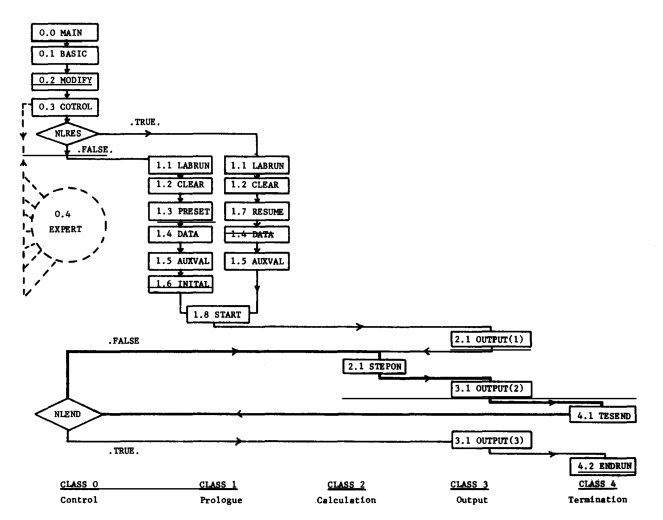
\includegraphics[width=0.9\textwidth]{../pics/cronos}}
\caption{Fig.~1 from ref~\protect\cite{Ch74Stan}, showing
the top-level design pattern. The thick line indicates
the main loop.\label{fig:cronos}}
\end{figure}

\Fig{olympus_diagn} shows a second pattern built around the \F{OLYMPUS}
library of modules such as {\tt MESAGE} and~{\tt HVAR}.
The library is of no intrinsic interest now because it is mostly
concerned with either timing or string handling. Nonetheless it is important
as an early example of `separation of concerns' to provide portability
between machines.  In the 1970s the local computing service
might well have had to implement the \F{OLYMPUS} library in machine-specific
assembly code.  Nowadays, computer languages have as standard very flexible
timing and string handling functions, that emerged out of a set of largely
ad hoc libraries like \F{OLYMPUS}.  Hopefully a similar upgrade path will 
ultimately be followed by HPC coding of for example array-based manipulations
that currently can only be implemented efficiently in an architecture-dependent way.

\begin{figure}
\centerline{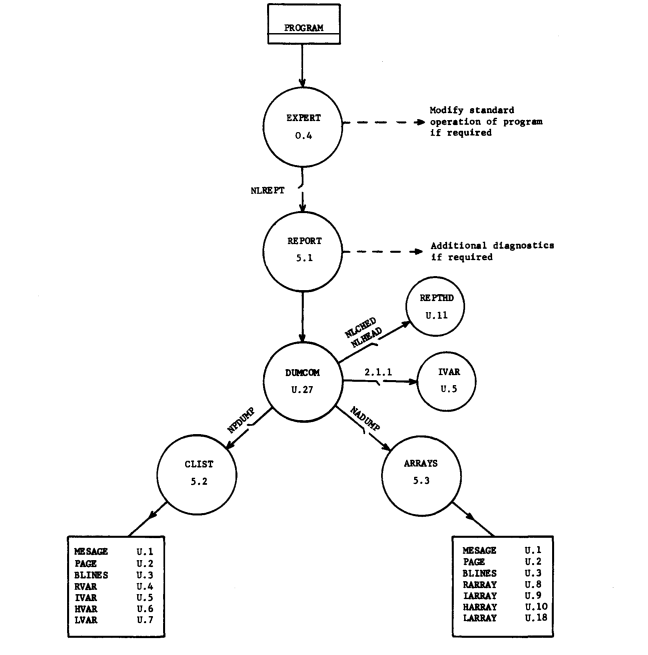
\includegraphics[width=0.9\textwidth]{../pics/olympus_diagn}}
\caption{Fig.~4 from ref~\protect\cite{Ch74Stan}, showing the
diagnostic design pattern, and indicating library routines
(with the ``U"~classification).\label{fig:olympus_diagn}}
\end{figure}

\subsection{\F{SMARDDA} Modules}\label{sec:smardda}
The U(nix)-\F{OLYMPUS} tools were developed from \F{OLYMPUS} in the late 1980s with the recognition that Unix$^{TM}$
was becoming the default operating system for scientific work. They represented a 
combination of the \F{OLYMPUS} framework above and C~shell scripts designed to enhance programmer
productivity, both at the individual level, by eg.\ 
accepting free format input of FORTRAN code and documentation, and at team level
by promoting use of standard data and calling structures, and indeed workflows.
The new Fortran standards emerging in the 1990s as Fortran~90 and Fortran~95 reduced
the need for many of the U-\F{OLYMPUS} features, Linux largely replaced Unix, and U-\F{OLYMPUS}
was not further updated. For Fortran~95 developments, emphasis switched
more on to promoting a coherent style, to exploit the object-oriented features
of the Fortran~95 language efficiently.  This style was eventually published in ref~\cite{fprog},
which includes templates for typical object complexities.

\paragraph{Physics and Scope}
The \F{SMARDDA} modules~\cite{Wa14b} are a 21st Century development of object-oriented software
in this style for magnetic fusion applications.  The \F{SMARDDA} modules
were originally developed for neutronics~\cite{Wa09a} and neutral beam duct design~\cite{Wa15}.
As a result of the latter, the basic \F{SMARDDA} algorithm was designed to be efficient both for
short ``rays" representing gyro-orbit segments as well as ``long rays" representing
neutrals and neutron paths, by combining two pre-existing algorithms, SMART and DDA.
Ionised particle trajectories in the ducts were treated using the well-known Boris
algorithm~\cite[\S\,4-7]{hockneyeastwood}.
In the subsequent development for fieldline tracing~\cite{Wa14b}, the fact that the magnetic field was likely to 
be a solution of the discretised Grad-Shafranov equation that was only second order accurate in mesh-spacing led to the 
implementation of a low order Runge-Kutta integration scheme for following the field. An adaptive
(Fehlberg or Embedded method RKF23) time-stepping scheme was used purely to avoid the problem of
selecting an initial time-step. Hence through a sequence of different applications,
software was developed capable of following over $100$~million particles on a desk-top in an application 
to back-scattering electron power deposition in the JET neutral beam ion source~\cite{Tu19Ions}
and over $2$~million fieldlines in an application to JET plasma-facing components~(PFCs)~\cite{Wa19}.

\paragraph{Framework}
The original \F{OLYMPUS} pattern of flow control was not needed by \F{SMARDDA}, 
on the grounds that restarts were unlikely to be necessary, so that the equivalent of
the Class~$0$ and Class~$1$ are all combined in a single program module that has a $1, 2, 3$ layout,
where in sequence order, $1$~is initialisation, $2$~is compute and $3$~is output and closedown.
Indeed, strict application of object-oriented principles associates the main loop with a class,
eg.\ the set of all triangles approximating JET PFCs which might receive power along
the fieldline through each barycentre.
The software was developed as a set of classes, each with its
own I/O and constructor/destructor functions as laid out in the templates
listed by ref~\cite{fprog}, and in one-to-one correspondence with the modules of
the software. This classes ranges from the generic, for logging error and warnings,
to the generally useful, for representing geometry, to the more fusion-specific
such as magnetic field representations, and ultimately the problem-specific, calculating
the power deposition in neutral beam ducts or on PFCs.
The program module sits at the apex of a hierarchy of classes, meaning
that it has to reference (`use') all classes in the hierarchy. It was
recently demonstrated~\cite{Wa19} that program modules themselves could be easily
modified to become classes referred to by a more encompassing program module.

Initially there was a library consisting of routines written in FORTRAN~77,
callable by modules written in Fortran~95. In time, it became clear that it would be
helpful to construct a library of Fortran~95 modules that could be used
by the different applications, see \Fig{layout}. Hence the \F{SMARDDA} modules have all
the features of a framework, excepting that the skeleton is modifiable within
the $1, 2, 3$ layout described above.

\paragraph{Documentation}
Regarding documentation, much was produced under contract to ITER intended for designers
who would use the software as a `black box', so-called user documentation. doxygen
is used as it fortunately acquired a significant capacity to model Fortran~95 
immediately prior to the documentation contract. However, doxygen does not
recognise the Fortran namelist feature which is the main way in which
control data is input, meaning that namelists have to be crafted into derived types.

\begin{figure}
\centerline{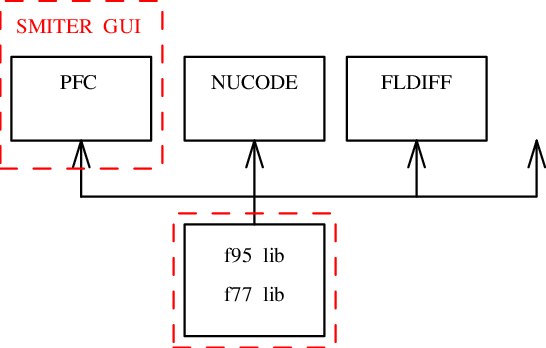
\includegraphics[width=0.7\textwidth]{../pics/layout}}
\caption{Library structure of the \F{SMARDDA} modules. The Fortran~95 (f95) library
contains modules used by one or more of application codes \F{SMARDDA-PFC},
\F{SMARDDA-NUCODE}, etc. (The parts of the software in red boxes form the kernel
of the ITER IMAS code~SMITER.)\label{fig:layout}}
\end{figure}


\subsection{FLASH}\label{sec:flash}


FLASH \cite{flashwebsite} is described:
\begin{quote}
{\it `The FLASH code is a publicly available high performance application code 
which has evolved into a modular, extensible software system from a collection 
of unconnected legacy codes.'}
\end{quote}

Dubey~et~al~\cite{Du09Exte} add to the description {\it `... a Massively-Parallel,
Multiphysics Simulation Code'}.  FLASH is a community astrophysics code; it has been a clear 
success in terms of uptake since its inception in Y2K - there are now over 1000 
citations on the FLASH website~\cite{flashwebsite}.


The code formed when legacy solvers (written in Fortran 77) were refactored 
into a formal software engineering framework.  Subsequent additions to the code 
have been driven by the physics requirements of the users; Dubey~et~al~\cite{Du09Exte} 
references in its title the code's {\it `Extensible Component-Based 
Architecture'}.

\paragraph{Physics and Scope}

Capabilities include compressible hydrodynamics, MHD, nuclear burning, 
equations of state, radiation, laser drive, fluid-structure interactions, and 
also particles, which may simply be non-interacting `tracer' particles.
Kinetics (represented by the Boltzmann equation) and 
gyrokinetics seem absent from the codebase.  Gravity (an always-additive and 
therefore long-range force) is clearly a pressing matter for astrophysics but 
is irrelevant for \nep; likewise any cosmolological / relativity physics. 
The codebase uses only rectilinear computational meshes.


\paragraph{Framework} 

The core algorithms are written in Fortran~90 and wrappers are written in~C.

The code is structured into components called Units (many of which implement a 
specific component of the physics capability; an example is particles) and the 
code for an individual Unit is demarcated using the Unix directory structure.  
A build includes only the Units needed for the problem in question.  The top 
level of a Unit's directory defines the API of the Unit.  Unit-private data is 
passed laterally by reference using accessor functions as needed.  Subunits 
allow alternative implementations and also give scope to shared data, avoiding 
proliferation of accessor functions.  Simulations are specified via a 
collection of config files included at various places in the directory 
structure: files lower down the hierarchy can override ones inherited from 
higher up.  Users can incorporate novel physics by adding a new Unit.  

The framework is object-oriented and encapsulates data; however, this is 
accomplished using the directory structure and a set of parsed config files 
(written in a domain-specific language), rather than using an explicit 
object-oriented language.  It is stated in \cite{Du09Exte} that this may be 
beneficial for portability.

Each simulation would appear to necessitate compilation of a new executable; 
the object-oriented character is strictly at compile (i.e. build) time and it 
seems the code must be rebuilt to change what the simulation does (excepting 
parameters read in by config files).

There is no GUI; user interface is via text files / command line.  Multiple I/O 
libraries are supported e.g. HDF5 and parallel netCDF (see \cite{Du09Exte}).

The workflow includes a test suite, which is run nightly.
There is an integrated unit test framework and a self-test suite for regression testing.  
An ensemble of quick-running examples has been proven by a user survey to be a popular feature.  

There is rigorous gatekeeping for non-internal extensions to the release version of the code, 
including a requirement for a specific unit test and a commitment to provide support.

The user community consists of mainly astrophysicists, but there are some other areas of application.
There is an email users' group, with support provided by experienced users and the developers.
The code is free on request; users may modify but not redistribute their own copies.
Documentation includes a User's Guide and also API description extracted using {\it robodoc}.
One interesting aspect has been user surveys, which
have provided insight into how the code was used and also 
indicated the most widely appreciated aspects of the code.
\cite{Du09Exte} cites feedback from close to 300 respondents, which gives
the top reasons for FLASH usage as
\begin{enumerate}
\item Adaptive mesh refinement (64\%)
\item Flexible (47\%)
\item  Good documentation (47\%)
\item  Availability of examples (43\%)
\item  Computationally efficient (37\%)
\item  Easy to Use (36\%)
\end{enumerate}


\paragraph{Summary}

FLASH is a true multiphysics code and incorporates fields and particles.  Its 
authors claim efficient operation up to tens of thousands of processors 
(\cite{Du09Exte} includes an example of 16 million particles running on 32,768 
nodes of IBM BG/L machine).  %Our anticipated scaling requirements exceed this.



Disadvantages are associated with the rather amphibious nature of the code: it 
uses build-time methods to achieve object-oriented features from 
non-object-oriented languages and so must be largely recompiled for each 
simulation; also, the code is written in more than one language.  Writing in 
Chapter~1 of \cite{carverhong}, the authors of the code state that the 
framework was chosen because the original physics capability was in Fortran and 
to refactor in an object-oriented language was not an option; it is also 
conceded that {\it `... FLASH ... has a big challenge in adapting for 
future heterogeneous platforms'}.  It appears the use of the code may have 
`peaked': there are only five publications listed from 2019 and ten from 2018; 
cf. 93 in 2010 \cite{flashwebsite}.


%\paragraph{Documentation}
%User's Guide.  API description extracted using {\it robodoc}.
%
%\paragraph{Workflow / release cycle}
%Nightly test suite.  Gatekeeping for non-internal extensions to Release.  
%Integrated unit test framework.  Self-test suite for regression testing.  Suite 
%of quick-running examples (proven, by a user survey, a popular feature).
%
%\paragraph{Community}
%Mainly astrophysics, but some other.  Email users' group (experienced users and 
%devs provide support).  User surveys.  Code free on request; users may modify 
%but not redistribute own copies.
%%



\subsection{Arcos}\label{sec:arcos}

The US Department of Energy (DOE) develops a suite of software for studying Earth Sciences.
Among these are Amanzi \cite{Mo14Aman,amanzi_repo} and The Advanced Terrestrial Simulator (ATS)\footnote{``formerly sometimes known as the Arctic Terrestrial Simulator'' \cite{ats_repo}} \cite{ats_repo}, a pair of codes which have been developed since 2012.
Amanzi solves for flow and reactive transport in porous media, to allow modelling of mineral and contaminant flow through rock and soil.
ATS adds the capability to solve effects from ecosystem hydrology, such as thermal processes, evapo-transpiration, surface energy balances, and vegetation modelling \cite{ats_repo}.
Both Amanzi and ATS are written in C++, using modern software engineering standards, and make extensive use of third party libraries such as Trilinos, PETSc and Hypre.
Both are open source and available on GitHub \cite{amanzi_repo,ats_repo}.

\paragraph{Framework}
To enable multiphysics simulations with Amanzi and ATS, the Arcos framework \cite{Co16Mana} was developed to couple the codes.
Arcos is a management system with three components, a process tree, a dependency graph, and a state/data manager.

The process tree formally describes the coupling hierarchy of the equation system to be solved.
Each leaf node is an equation, while each internal node couples children together to form systems of equations.
Each node provides the same interface to its parents, so that equations and systems of equations may be grouped recursively into a hierarchy.
This approach merely formalizes the natural structure existing in most multiphysics systems and codes.
However, using an explicit, general and dynamically-formed structure means much of the coupling can be automated.
It also allows domain specialists to focus on developing single components without fear of side effects in other parts of the model hierarchy.

The nodes in the process tree only perform administrative work;
actual computational work on the equations is delegated to \emph{evaluators}.
These evaluators manage one of three kinds of variable, namely
1) independent variables, user-provided functions of the coordinates,
2) primary dependent variables, functions of independent variables for which an equation has to be solved; and
3) secondary dependent variables, functions of other dependent variables.
The evaluators are stored in a directed, acyclic graph (DAG) that describes the relationship between variables.
Independent and primary dependent variables are leaf nodes in the DAG.
All other nodes represent secondary dependent variables, with the directed edges pointing to their dependencies.

While evaluators perform work, they do not store any data (beyond simple metadata).
Instead, evaluators access data via the data/state manager, which stores data and controls access to it.
This abstracts the physical equations away from the data management, allowing each component to be developed by the relevant expert.

\paragraph{Modularity}
Arcos' approach is extremely fine-grained.
Unlike most scientific software which is modular at the level of equations, Arcos is modular at the level of terms in an equation.
This has the following advantages.
Firstly, models become more easily interchangeable - for example, pressure depends on temperature and density (in non-isothermal models), or just density (in isothermal models). The evaluator representing pressure will either have or not have an edge in the DAG pointing to temperature, depending on the model.
However, other parts of the framework depending on pressure will not need to know whether the model is isothermal.
This allows for tight coupling of models, with optimization via lazy evaluation of variables.
The dependency graph also means that programmers do not need to manually track and edit code to account for dependencies in different models, reducing bugs and code duplication.
This also makes it relatively easy to implement new models at any part of the hierarchy.

The fine-granularity also means that Amanzi/ATS is very amenable to unit testing.
Unit testing is difficult in less granular codes, as to test an equation, it must often also be initialized with a mesh, a solver and other components.
As the evaluators in Arcos represent a single term, not an equation, and as they hold no data themselves, they are far easier to isolate and test. 
In addition to a unit testing suite, Amanzi/ATS developers also provide a suite of integrated tests, which double as example problems to aid new users. 

\paragraph{Performance portability}
It is difficult to make statements about performance given the range of models covered by Arcos.
However, the Arcos framework has a number of features that are favourable for performance portability.
Firstly, by using well-supported solver libraries like Trilinos, Arcos leverages improvements in numerical algorithms with minimal efforts.
Secondly, by having a fine-grained heterogeneous structure, Arcos is a good candidate to take advantage of emerging ``coarse task'' runtime environments.
Finally, the nature of evaluators -- stateless functors with no side effects -- makes Arcos a good candidate for use across a variety of platforms. 
Evaluators abstract what is done to data from how and where it is done, making it a good framework in which to implement multiple parallelization paradigms (e.g. MPI, OpenMP, CUDA etc.) without intrusion onto the physics code. 

\paragraph{Summary}
The distinctive features of the Arcos framework are its use of a formal structure to describe the equation hierarchy, and its very fine-grained modularity, where every term in an equation is treated as an independent object.
This enables a number of features that are desirable in ExCALIBUR.
Firstly, the formal graph structure automatically handles dependences in an equation hierarchy, making it easier to implement different models without introducing bugs or code repetition.
Secondly, it enables a separation of concerns, with domain specialists able to modify code sections in isolation.
Finally, the framework enables performance portability, as the heterogeneous code structure is well-placed to exploit emerging exascale technologies.

\subsection{BOUT++}\label{sec:bout}


BOUT++ \cite{bout431,boutwebsite,boutrepo} describes itself as
\begin{quote}
a framework for writing fluid and plasma simulations in curvilinear geometry. The design is modular, with a variety of numerical methods and time-integration solvers available that can be chosen at runtime. BOUT++ is primarily designed and tested with reduced plasma fluid models in mind, but it can evolve any number of equations, with equations appearing in a readable form. The code is opensource, licensed under the LGPL, and is available from https://github.com/boutproject/BOUT-dev
\end{quote}

\paragraph{Framework}

BOUT++ is a multi-block finite difference / volume PDE solver written in C++, with parallelisation using MPI and/or OpenMP.
GPU acceleration is under development.
There are optional dependencies on a variety of third-party libraries such as FFTW, SUNDIALS, PETSc, SLEPc. I/O is via netCDF or HDF5. 

The core of BOUT++ is a library of functions relevant to plasma simulation in 3-D curvilinear geometry, such as differential operators, definitions of tokamak domains and magnetic geometries (e.g. single/double null), and common boundary conditions. 
BOUT++ also provides routines for integrating equations in time and for inverting elliptic operators.

As a library, BOUT++ does \emph{not} specify the equations to be solved.
These are specified by the user in defining their ``PhysicsModel'', a class that provides ``init'' (initialization) and ``rhs'' (right-hand side) functions.
The class is then passed to BOUT++, that is, the user cedes control of the workflow to the library.

In addition to the core library, the BOUT++ project also provides Python utilities for grid generation, post-processing and plotting in tokamak geometries.

\paragraph{Domain-specific language}
The BOUT++ library routines provide a domain-specific language (DSL), allowing the user to specify equation systems in a human-readable fashion.
For example, the wave equation (for amplitude $f$ and velocity $g$ and unit wavespeed) may be written in the user's physics model as
\begin{align*}
  \mathtt{ddt(f) = Grad\_par(g);}\\
  \mathtt{ddt(g) = Grad\_par(f);}
\end{align*}
This allows physics models to be implemented in BOUT++ with minimal effort, allowing rapid prototyping.
It also means there is a very low bar to entry for new users/non-programmers, and physics models may be implemented with no knowledge of the underlying numerics -- for better or worse!

\paragraph{Performance}
BOUT++ is a versatile framework that may be run across the spectrum of computing system sizes, from laptops to large HPC systems.
BOUT++ is currently deployed on Archer (UK Tier-1) and Marconi (Tier-0), among others, and scales to ${\cal O}(1000)$ cores for typical problem sizes.

Two of the three dimensions are parallelized with MPI, while all dimensions are parallelized with OpenMP (recasting the 3-D arrays local to an MPI rank as a flat vector).
The MPI parallelization in one of the dimensions and the OpenMP parallelization were retrofitted -- the anisotropy of plasma in strong magnetic fields meant that in early simulations the resolution used in all-but-one of the dimensions was not sufficiently large to merit parallelization.

\paragraph{Software sustainability and community}
BOUT++ is freely available via the public Github repository \cite{boutrepo}, and is licensed under the LGPL. Development is done in public, with regular feedback from community members.
%
BOUT++ uses a development model similar to gitflow, with a stable \texttt{master} branch and a development \texttt{next} branch. \texttt{next} forms the basis for major and minor releases, so new features are introduced into \texttt{next}, while bugfixes are introduced into both \texttt{master} and \texttt{next}.
Both these branches are protected, and new code only enters via a pull request, which requires code review and approval from a maintainer before being merged.
Travis CI is used to automatically run a comprehensive suite of both unit and system (integrated) tests on every push to the Github repository. Creation and update of pull requests triggers additional tests. Several build configurations are tested, including optimised builds, different compilers and Linux distributions, and linking against various optional third party libraries.

New releases are recorded on Zenodo, allowing each release to have a citable Digital Object Identifier (DOI).
Having a DOI for each version is important for reproducibility of scientific results, but producing an accompanying paper for releases simply to obtain a DOI may be an incommensurate amount of work, or not deemed of sufficient interest to be publishable.
Reproducibility is further aided by the output of each run recording the git commit hash and the state of the repository (``clean'' or ``modified'').

Documentation is automatically built from doxygen comments in the source code and hosted online at ReadTheDocs \cite{boutreadthedocs}, while bug reports and community feedback can be done via the Github issue tracker or the BOUT++ Slack workspace.

Hands-on training led by the maintainers is provided for new users at annual workshops, where users can also present their research and discuss new and future code development and features. Research and code development can also be presented at the monthly user meetings, held via video conference.

\paragraph{Summary}

BOUT++ is a versatile, easy-to-use and reasonably-performative framework.
It successfully implements a ``separation of concerns'' between the roles of user and developer.
For users, the DSL allows models to be written in human-readable form, with simple access to complicated geometry-dependent operators.
Different numerical methods for discretization and time-integration may be selected at run-time.
This means there is a low barrier to entry for prototyping models, and for running simulations on Tier-0/Tier-1 HPC systems.
For developers, the source code is freely available on the repository, along with contribution guidelines.
There is also an active community of developers around the repository, Slack channel and BOUT++ User Group meetings.

Not all features of BOUT++ are appropriate for ExCALIBUR projects however.
BOUT++ emphasizes flexibility rather than performance. 
One example of this is in the domain specific language where BOUT++ favours a clear interface for the DSL, over optimal performance for any one set of systems.
Requiring that operators (such as \texttt{Grad\_par(g)} above) are independent objects means that the right-hand side functions are concatenations of objects, each being relatively small kernels of work. 
Joining these into a single loop would require introducing a global index and an outer loop, so operators would be written \texttt{Grad\_par(g)[i]}.
While this could be circumvented with code generation techniques, this has not yet been implemented, and BOUT++ developers favour the cleaner interface to raw performance.

There is also an issue with political control of the users' physics models. 
The library nature of BOUT++ allows users to develop sophisticated models (e.g. STORM (from CCFE), Hermes and SD1D (from the University of York), plus other models from other individuals/institutions), which themselves require infrastructure like repositories, testing and contribution guidelines. 
These models have varying degrees of independence from the core BOUT++ framework.  
Hermes and SD1D are developed by the core BOUT++ developers; STORM is developed in collaboration with BOUT++ developers; in contrast, the source code for physics modules belonging to other institutions are not usually available to BOUT++ core developers.
    Yet all of these may be presented in papers or at conferences as being ``BOUT++''.
    This is a reputational risk to the BOUT++ project.
    It has been mitigated to some extent by bringing some physics modules into the main repository and testing them, and by endeavouring to collaborate as widely as possible.

\subsection{Nektar++}\label{sec:nektar}


Nektar++ is described (\cite{nektarwebsite}):
\begin{quote}
{\it `Nektar++ is a tensor product based finite element package designed to allow one to construct efficient classical low polynomial order h-type solvers (where h is the size of the finite element) as well as higher p-order piecewise polynomial order solvers.'}
\end{quote}
The code is opensource under the MIT licence.  
It is modern and object-oriented, with the initial release dating from 2006.

\paragraph{Physics and Scope}

Nektar++ is a spectral / hp element framework for a range of PDEs, which can be hyperbolic, parabolic, or elliptic.
The code includes pre-written solvers for acoustic, advection-diffusion-reaction, cardiac electrophysiology, compressible flow, incompressible Navier-Stokes, linear elasticity, pulse wave, and shallow water problems.
The underlying method can be continuous or nodal discontinuous Galerkin.
There are the options of implicit, explicit, or IMEX time-stepping (though availability depends on solver choice).

Nektar++  does not currently support particles or any Boltzmann-type equations,
although for example the treatment of particle motion in spectral / hp elements
is described in the textbook~\cite{karniadakissherwin}.

%The current physics scope does not extend to particles or Boltzmann-type equations (rather, it is a generic PDE framework supporting up to 1 time and 3 space).

The solvers can be coupled to provide multiphysics capability.  
An MPI coupling implementation consists of a smooth interpolating field layer that is receiver-centric in that the receiver is provided with pointwise field data from the sender (then to be resolved to the local basis).  
Data transfer is handled using the CWIPI library~\cite{cwipiwebsite,Ca19Test}.  
This framework can couple different Nektar++ solvers, or couple one such to a separate application.

\paragraph{Framework} 

Nektar++ uses a modern object-oriented C++ framework \cite{Ca15Nekt}.  Multi-threading is via MPI.

The framework is multi-layered in that there is a structured hierarchy of C++ components (much of the structure is evident in the directory structure of the downloaded source code) and the code structure mirrors the mathematical formulation (see library descriptions below).  
The time-steppers are agnostic to the FEM/solver details and the solvers share much of the underlying FEM codebase.  
Solvers inherit from base classes, for example one for unsteady flows.

The implementation is partitioned into six libraries, organized into utilities (parallel communications, DFT, maths routines), reference elements, physical elements, domain geometry and mesh, global field data operations and solver base classes.

There is no GUI; input is via XML file (mesh, solver, parameters, boundary conditions); output is via file (HDF5 is supported).  
Tools are provided for converting input meshes from popular formats ({\it NekMesh}, which also can make a mesh `higher order', meaning the inclusion of curved-sided elements) and for converting the output to popular formats ({\it FieldConvert}).  
Note that the latest version \cite{Mo20Nekt} supports input meshes in HDF5 format in order to avoid the need for a single process to read the entire mesh during setup.

The code is designed to run on anything from a single desktop up to many thousands of processor cores.

The development workflow involves a monthly stable release.  
There is an extensive testing framework.

The focus of the user community seems primarily engineering and biomedical.  
The entry barrier is lowered by the availability of a precompiled binary in addition to the source code.  
Documentation includes a User's Guide and API description extracted using {\it doxygen}.
The code is under active development by groups at the University of Exeter, Imperial College London
and the University of Utah.


\paragraph{Summary}

Nektar++ has a well-designed framework, is written in a clean way in a modern, object-oriented language, and it looks relatively easy to add new solvers.  
The option to download a ready-built code (as alternate to the full source) provides an easy entry point for new users for whom there is no need to modify the code.  Nektar++ has proven scaling up to tens of thousands of processors.

The caveat is that the existing framework requires new
physics to be described by PDEs in up to 1+3 dimensions, ie.\ maximally time-dependent
in $3$ space dimensions, and
solved using by the restricted set of supported finite-element methods.

There does seem to be some `price of admission' in terms of user expertise; for example, it is not clear what guidance user gets regarding the maximum timestep in explicit methods to avoid violating the Courant stability limit.

%\paragraph{Documentation}
%User's Guide.  API description extracted using {\it doxygen}.
%
%\paragraph{Workflow / release cycle}
%Stable releases monthly.  Extensive testing framework.
%
%\paragraph{Community}
%Focus seems to be engineering / biomedical.  Under active development by groups at Imperial College London and the University of Utah.  Community blog.  Precompiled binary available in addition to source / {\it CMake}.



%



% ---------- JOREK Sub-section
\subsection{JOREK}\label{sec:jorek}


JOREK \cite{JOREK,Huysmans2007,Czarny2008} describes itself as
\begin{quote}
The nonlinear extended magnetohydrodynamics (MHD) code JOREK resolves realistic toroidal X-point 
geometries with a $C^1$~continuous flux-surface aligned grid including main 
plasma, scrape-off layer and divertor region. It is based on robust fully 
implicit numerics, and includes sheath boundary conditions, resistive wall 
effects, two-fluid effects and neoclassical flows, and particle models.

The well-established physics and numerics community around JOREK has strong 
connections to the relevant experiments, ITER Organization and the respective 
ITPA Topical Groups.
\end{quote}

%\paragraph{Features}
%
%List of main features:
%\begin{itemize}
%    \item Fortran code
%    \item IO: HDF5
%    \item Fully implicit schemes
%    \item $G^1$~continuous Finite-elements
%    \item wide variety of physics applications
%    \item regression test suite - automated on ITER cluster
%    \item Documentation via wiki
%    \item Visualisation using .vtk (eg. Paraview, Visit)
%    \item Infrastructure on ITER platform
%\end{itemize}

\paragraph{Numerics}

JOREK is an implicit finite-element code written in Fortran, with 
parallelisation using MPI and OpenMP. It uses a 2-D grid of bi-cubic Bezier 
elements in the poloidal plane, and Fourier harmonics in the toroidal 
direction. The fully implicit timestepping scheme leads to a linearised
system which is solved by using pre-conditioned GMRES,
with a pre-conditioner built by solving independently each individual Fourier 
harmonic matrix. The code has dependency on a sparse-matrix solver, which at 
present can be one of MUMPS~\cite{MUMPS}, PASTIX~\cite{PASTIX} or STRUMPACK~\cite{STRUMPACK}.
The time-step solver includes the options of Euler, Crank-Nicolson and Gear schemes.

The 2-D poloidal grid is made of quadrangular bi-cubic Bezier elements, which 
are aligned to the magnetic flux-surfaces, and which can be extended to 
arbitrary wall surfaces, applicable to any tokamak \cite{Pamela2019}. A coupled 
free-boundary module of JOREK-STARWALL \cite{Hoelzl2012,Artola2018,Artola2020} 
is also available to look at resistive-wall effects, and disruptions of a VDE 
nature (Vertical-Displacement-Event). New geometrical representations are also 
under development for Stellarators.

The I/O of JOREK is done using HDF5 format. A large number of post-processing 
tools are also available to look at various aspects of simulation results, like 
fast-camera imaging, Infra-Red thermography for wall and divertor fluxes, 
line-profiles, integrals etc.

\paragraph{HPC}

The JOREK code typically requires an HPC architecture to run advanced cases. 
Although simple, small test-cases can be run on a laptop, high-resolution 
requires several thousands of cores on HPC clusters.

\paragraph{Physics}

There are a number of physics models addressing a wide range of tokamak 
applications. The base models are reduced- and full-MHD models. Extended models 
include
\begin{enumerate}
    \item two-temperature fluid models
    \item two-fluid (diamagnetic) model
    \item neutrals fluid model: applied to disruption mitigation and divertor 
detachment
    \item impurity fluid model: applied to disruption mitigation
    \item kinetic particles pusher: applied to runaway electrons, impurity 
transport
    \item relativistic electron fluid model: applied to runaway electrons
    \item coupled fluid-particles model: applied to TAE's, detachment, ITG 
turbulence
\end{enumerate}

\paragraph{Development}

The JOREK code is hosted at ITER, using the integrated platform for code 
developments. The main features used from the platform are
\begin{enumerate}
    \item Jira: used to raise, discuss, resolve and track issues from the 
community, addressing both physics and numerical aspects of the code
    \item Bitbucket: used to manage git branches, merges and pull-requests
    \item Bamboo: used to schedule automated regression tests for 
pull-requests
\end{enumerate}


\paragraph{Community}

The principal coordinator of the JOREK community is Matthias Hoelzl, based in 
Garching, Germany. The main (initial) author of the code is Guido Huijsmans, 
based at CEA, France, and at Eindhoven University, the Netherlands. There are a 
number of code-developer and code-users throughout Europe, Asia and the USA.

Communication is organised via a wiki linked to the 
website~\cite{JOREK} which is restricted to a team of registered users and developers.
Meetings of team members typically occur several times per month, to 
present and discuss various projects and developments. A general meeting is 
held once per year for one week. There are several mailing lists, eg.\ one for the 
entire community, and a helpdesk which includes only expert developers.
The restricted JOREK wiki includes a variety of code documentation, ranging from physics 
equations and other material useful for developers, to user-guides for various 
aspects of the code etc.


\paragraph{Pros}

\begin{itemize}
  \item High standards of software development
  \item Well-organised community
  \item Wide range of applications
  \item New physics models relatively straightforward to implement
\end{itemize}

\paragraph{Cons}

\begin{itemize}
  \item Scaling: like all fully-implicit codes, JOREK requires the solving of 
large sparse matrices, which necessitates large amounts of memory
  \item At present only one type of finite~element is available
  \item Performance dictates new developments, at the detriment of modularity
\end{itemize}




\subsection{Comparative Table for Different Frameworks}\label{sec:compare}
\begin{table}[h]\label{tab:assess}
\begin{center}
\caption{Metrics for frameworks described in detail.}
\begin{tabular}{|p{2.0cm}|p{4.0cm}|p{2.2cm}|p{1.6cm}|p{2.4cm}|p{1.6cm}|p{1.6cm}|}
\hline
Framework & Physics & Language(s) & Docum'n & Maintenance & User     &  UKRI \\
          & Areas   &             & Qualty  & years approx    & Level(s) &  skills  \\
\hline
OLYMPUS & All & FORTRAN & 5 & 50 & 5 & 5  \\
SMARDDA & Surface interactions & Fortran~95 & 4 & 10 & 1,2,5 & 5  \\
FLASH & Astrophysics & Fortran 90, C & 5 & 20 & 1-5 & 3 or 4(?) \\
BOUT++ & Tokamak Edge/Scrape-off layer & C++ & 4 & 20 & 2,4,5 & 5 \\
Nektar++ & Fluids FEM & C++ & 5 & 14 & 1-5 & 5\\
Arcos & Earth sciences & C++ & 4 & 10 & 2,4,5 & 1 \\
JOREK & Tokamak Edge & FORTRAN & 4 & 10 & 4 & 4,5 \\
\hline
\hline
\hline
\end{tabular}
\end{center}
\end{table}

\begin{enumerate}
\item Documentation Quality
\begin{itemize}
\item[1] Limited documentation online
\item[2] Published papers describing use
\item[3] Extensive documentation online
\item[4] Published papers describing code in detail
\item[5] Linked textbook
\end{itemize}

\item Level of user/developer
\begin{itemize}
\item[1] Application program level, only changing physics parameters.
\item[2] Programmer in high level language such as Python.
\item[3] As 2, but occasional programmer in C, C++ and/or FORTRAN.
\item[4] Real programmer using mostly C etc.
\item[5] Developer
\end{itemize}

\item UKRI skills available
\begin{itemize}
\item[1] No evidence
\item[2] Ability to use code
\item[3] Ability to use code and understand limitations
\item[4] Demonstrated ability to modify code
\item[5] Significant part of code written in UK
\end{itemize}

\end{enumerate}

